
\documentclass[a4paper,openright,11pt,oneside]{book}
\usepackage[spanish]{babel}
\usepackage{graphicx}



\begin{document}
	\begin{titlepage}
		\begin{center}
			\vspace*{-1in}
			Universidad de La Habana \\
			Facultad de Matemática y Computación \\
			\vspace*{0.15in}
			\begin{figure}[htb]
				\begin{center}
					
\includegraphics[width=3cm]{./Graphics/uhlogo.pdf}
				\end{center}
			\end{figure}
			
			\vspace*{0.3in}
			\begin{large}
			\textbf{Selección automática de casos de prueba con aprendizaje de la medida de calidad} \\
			\end{large}
			\vspace*{0.6in}
			Autor: \textbf{Marcel Ernesto Sánchez Aguilar} \\
			Tutores: MsC. \textbf{Ludwig Leonard Méndez}, Lic. \textbf{Carlos Fleitas Aparicio}
			
			\vspace*{0.4in}
			Trabajo de Diploma presentado en opción al título\\
			Licenciado en Ciencia de la Computación
			
			\vspace*{0.5in}
			Septiembre de 2020
			
		\end{center}
	\end{titlepage}
\chapter*{Dedicatoria}
A mi maravillosa familia de la cual me siento muy orgulloso, en especial de mis padres.

\chapter*{Agradecimientos}
	A mis padres, que me han dado la educación que tengo y han forjado todo en mí. Son mi fuente de inspiración y mi ejemplo a seguir.
	
	A mi abuelo, con el cual tengo buena parte de los recuerdos más traviesos y hermosos de mi niñez. Ojalá yo pueda llegar a ser para mis nietos tan importante como lo ha sido Abu para mí.
	
	A mis dos abuelas, que tanto me cuidaron y mimaron. Por cumplir su rol de abuela a la perfección y darme tantos recuerdos inmejorables.
	
	A mi bisabuela Mima, que me picaba los caramelos para que no me ahogara de niño.
	
	A mis tíos Liss y Ale, los quiero un montón y son los mejores médicos del mundo.
	
	A mi primo Derly, que lo quiero como a un hermano. Que ha sido mi amigo, mi compañero de juego, mi rival; para el cual hago para que se sienta orgulloso de mí.
	
	A Dios por permitir que toda mi familia sea testigo de este momento.
	
	A mis amigos de la infancia Yorlan y Kevin, que juntos hemos vivido momentos épicos y no los cambio por nada en este mundo, con los cuales he reído en las buenas y sufrido en las malas.
	
	A mis profesores de la primaria, que me enseñaron a leer y escribir, que me inculcaron el amor por la matemática y la pasión por el ajedrez.
	
	A todos los profesores que me han educado y enseñan con una pasión que da gusto y enamora. He tenido la suerte de conocer a muchos, como a mis abuelos en Física y Química, a Disodado en Histoira, a María del Carmen en Biología, a Enma en Matemática, a María Antonia en Español y a Somoza en Discreta.
	
	A mis profesores de la universidad que tan bien me enseñaron y prepararon para ser un profesional.
	
	A mis compañeros de universidad con los cuales me divertí, estudié y estresé en la travesía de la carrera. 
	
	Al profesor y tutor Ludwig por permitirme ser alumno ayudante y vivir la maravillosa experiencia que resultó.
	
	Al profesor, compañero de trabajo, amigo y tutor Carlos; con quien aprendí de bases de datos, de cómo dar clases y a quien debo mucho y agradezco por el apoyo que me brindó durante la tesis, su ayuda fue vital.


\chapter*{Opinión de los tutores}\label{chapter:supervisor_opinion}
\addcontentsline{toc}{chapter}{Opinión de los tutores}
	
	La evaluación de la correctitud de un algoritmo y su codificación es un proceso variado y en muchos casos, complejo. El algoritmo debe devolver la respuesta esperada de cada entrada y resolver el problema para el que fue creado. De igual manera, es muy importante que la codificación del mismo refleje efectivamente su diseño. A pesar de ser una cuestión vital desde los inicios de la Computación, cobra especial significación en el contexto de la enseñanza de la Programación. En el proceso de aprendizaje son muy comunes los errores de diseño e implementación de algoritmos. En particular en la Facultad de Matemática y Computación, el sistema de evaluación de la asignatura Programación, impartida a estudiantes de primer año de la carrera de Ciencia de la Computación, comprende cinco exámenes de laboratorio. Estos implican la resolución de problemas computacionales en un ambiente controlado pero lo más similar posible al contexto real al que se enfrentarán los estudiantes en sus vidas profesionales. Este empeño supone una gran carga de trabajo para el claustro de profesores. Actualmente existe una solución automatizada que evalúa las implementaciones dado un conjunto de casos de prueba pero que resulta insuficiente, pues requiere de la definición manual de los casos y la intervención de los profesores para garantizar que las calificaciones sean justas. Es un proceso tedioso y, en según el caso, muy difícil de realizar.
	
	En este escenario se enmarca el trabajo de diploma de Marcel Ernesto Sánchez Aguilar. Ofrece una propuesta para la selección automática de casos de prueba con aprendizaje de la medida de calidad. Éste es un problema extremadamente complejo que pertenece al dominio de la Optimización Combinatoria. Además, las particularidades de los problemas a los que se aplica hacen que el aprendizaje no se comporte de la misma manera y la propuesta deba adaptarse a espacios de búsqueda muy diversos. Para ello, el estudiante debió consultar el estado del arte en el campo y seleccionar, dentro de las múltiples herramientas de solución, las más adecuadas. Su trabajo incluyó la identificación y adaptación de algoritmos meta-heurísticos para ser empleados en una gran variedad de escenarios, así como la comparación objetiva de los mismos respecto a su desempeño y potencialidades.
	
	
	Otro de los desafíos de la propuesta lo constituyó la búsqueda de exámenes y conjuntos de casos de prueba apropiados para la experimentación. Marcel se encargó de la generación automática de casos de prueba con fines del enriquecimiento de los conjuntos para el análisis. Éste es un proceso imprescindible para la investigación pero que excede el alcance de la misma y su contenido bastaría para otras tesis. 

	
	Igualmente, elaboró una propuesta de software vinculada a la solución automatizada existente que permite darle continuidad al trabajo realizado en el colectivo. Sin embargo, la generalización del enfoque de la solución permite aplicarla en cualquier proceso de evaluación por casos de prueba. Los resultados presentados avalan el desempeño del trabajo y abren nuevas posibilidades para el futuro. Este proyecto relacionó áreas como la Optimización, la Inteligencia Artificial, la Programación y la Ingeniería de Software.
	
	
	Marcel es un estudiante responsable, dedicado y creativo. La tesis requirió de una gran capacidad de ingenio para la propuesta de alternativas ante los problemas presentados, así como de abstracción para comprender conceptos complejos. En el trabajo sistematizó conocimientos adquiridos durante toda la carrera y otros no abordados en la formación básica, pero tratados con igual rigurosidad. Mostró su habilidad para llevar a cabo una investigación científica de manera coherente y expresar su desarrollo en una memoria escrita que cumple con los requisitos de calidad. Su vinculación con el colectivo de Programación data de varios años. Tuve el placer de compartir el aula con él mientras fue Alumno Ayudante de Programación y su apoyo fue vital en el desarrollo de las clases. Tiene una inclinación natural por ayudar a los demás. Su preparación, apoyo entusiasta e interacción con los estudiantes fue inmejorable. Igualmente, como su profesor, pude constatar la calidad de su desempeño. Reúne todas las cualidades y el conocimiento para ser un excelente profesional y le auguramos una carrera muy prolífica.
	
	\vspace{1cm}
	
	\begin{center}
		\emph{Lic. Carlos Fleitas Aparicio} \hspace{15pt} \emph{MSc. Ludwig Leonard Méndez} \\
		Facultad de Matemática y Computación \\
		Universidad de La Habana    
	\end{center}

\tableofcontents
	

\chapter*{Resumen}
	La confección de los casos de prueba para evaluar un algoritmo, a menudo es tarea difícil. Es necesario cubrir varios aspectos sin sobre incidir de más en alguno. Además, muchas veces se requiere de tener un conjunto representativo de casos  para que, a pesar de fallar en algún aspecto, se considere de aprobada la solución en algún examen.
	
	Dependiendo del problema, los evaluadores confeccionan un conjunto de casos tratando de que al menos esté representado el universo de los mismos, con la aspiración de lograr una evaluación justa. Esto es algo que resulta de gran complejidad, pues existen muchos detalles que, por omisión, pudieran traer una mala calificación.
	
	Sin embargo, el implementar una solución correcta o el percatarse de los errores más comunes es mucho más tratable. En este trabajo se propone una solución a esta problemática. Teniendo el criterio de un especialista que provea una solución que sean de una calidad especificada, se confeccionará un conjunto representativo de casos de prueba para evaluar un algoritmo.
	
%	 a partir de un generador de estos. Lo cual representaría una mejorar sustancial en el tiempo invertido por los evaluadores en el diseño de los casos de prueba, en su lugar han proveer implementaciones correctas; algo con que es usual contar. Además, se evitarán errores comunes en la generación de casos en aras de una evaluación más imparcial.
%	Para ello se abordan métodos metaheurísticos en la resolución de problemas de optimización combinatoria. \\
	
	\textbf{Palabras clave:} casos de prueba, algoritmo, conjunto representativo, solución de calidad.
	
\chapter*{Abstract}
	Making the test cases to evaluate an algorithm is often a difficult task. It is necessary to cover several aspects without over-influencing any. In addition, many times it is required to have a representative set of cases so that, despite failing in some aspect, the solution is considered approved in some examination.
	
	Depending on the problem, the evaluators make a set of cases trying to at least represent their universe, with the aspiration of achieving a fair evaluation. This is something that is highly complex, as there are many details that, by default, could lead to a bad rating.
	
	However, implementing a correct solution or noticing the most common mistakes is much more treatable. In this work a solution to this problem is proposed. Having the criteria of a specialist who provides a solution that is of a specified quality, a representative set of test cases will be made to evaluate an algorithm.
	
	\textbf{Keywords:} test cases, algorithm, representative set, quality solution.

\chapter*{Glosario}
	\begin{itemize}
		\item Aplicación: Sistema computacional que tiene como objetivo servir de herramienta a uno o varios usuarios en la realización de diversas tareas.
%		\item Aplicación de Consola: Es aquella que se ejecuta en una ventana mediante líneas de comandos.
		\item Software: Conjunto de programas y rutinas que permiten a la computadora realizar determinadas funciones.
		\item Casos de prueba: Conjunto de elementos de entrada que se utilizan para evaluar un programa.
		\item Algoritmo: Secuencia ordenada y finita de operaciones que permiten resolver un problema.
		\item Correctitud de un algoritmo: Se dice que un algoritmo es correcto si resuelve el problema para el cual fue diseñado, si produce la salida deseada acorde a la entrada suministrada y si termina en un tiempo admisible.
	\end{itemize}
	
\chapter{Introducción}

	La Ciencia de la Computación estudia los fundamentos teóricos de la información y la computación \cite{montero2017computacion}, así como su aplicación en la implementación de sistemas computacionales en correspondencia con el desarrollo vertiginoso de la propia ciencia y las tecnologías computacionales. El origen de esta ciencia es anterior a la invención del primer computador moderno, pues desde la antigüedad han existido procedimientos y algoritmos para realizar cómputos, solo que estos eran llevados a cabo por personas y no por un ente digital. Gracias a los trabajos de Alan Turing \cite{Turing} -considerado el padre de esta ciencia- y otros investigadores, se abrió el camino a nuevas ramas como la computabilidad y se profundizó en otras como la Inteligencia Artificial.
	
	Hoy en día la computación ayuda al hombre en casi todas las áreas y muchas tareas que antes se hacían de forma manual, se realizan ahora mediante un equipo de cómputo. Sin embargo, expresar en términos de calidad el buen funcionamiento de un software \cite{lopez2016definicion} resulta complejo. Para ilustrar el concepto de calidad de manera más profunda, es necesario considerar algunos aspectos fundamentales como son: solidez, exactitud, completitud, mantenibilidad, reutilizabilidad, entre otros.
	
	La aceptación de cualquier software pasa siempre por la lógica detrás del código y su correcta implementación. Esto es fundamental para el buen funcionamiento de cualquier programa. Un buen diseño de la misma puntúa de manera favorable el criterio de calidad, pero es difícil de medir, pues están estrechamente ligados y muchas veces no se sabe a simple vista dónde hay un fallo. Una buena lógica y un mal desempeño del código o viceversa, empañan el funcionamiento del programa. Sería ideal poder discernir entre uno, otro u ambos a la hora de analizar un error.
		
	\section{Contexto del problema}
		
		En la Facultad de Matemática y Computación de la Universidad de La Habana, los estudiantes de primer año que cursan la asignatura de Programación de la carrera Ciencia de la Computación se enfrentan a tres evaluaciones parciales y a una prueba final. Estos exámenes tienen la peculiaridad de que se realizan a través de un equipo de cómputo. Una vez entregadas las soluciones digitales (códigos) de los estudiantes al problema propuesto, se procede a evaluar las implementaciones de los mismos. El proceso de calificación de un examen en ninguna asignatura es trivial, por ejemplo, muchas veces lo que separa un ``buen"\ $3$ (a veces denominado $3^+$) de un ``mal"\ $4$ (o $4^- $) es la subjetividad del evaluador. En la práctica de esta asignatura en específica puede darse el caso de dos estudiantes con el mismo porciento de casos aceptados pero distinta nota debido a la dificultad de los casos fallidos, o con la misma nota pero porcientos distintos debido a la calidad del diseño presentado. Esto es algo extremadamente difícil de definir formalmente, pues esa subjetividad depende de los objetivos a vencer en las asignaturas y de experiencias en la enseñanza.
		
		Otro aspecto a señalar en estas pruebas particulares, es que la evaluación no se realiza directamente sobre los códigos de los estudiantes. Profesores de la asignatura se empeñan en confeccionar casos de prueba representativos que puedan dar una medida de la correctitud del algoritmo propuesto. La anterior tarea puede resultar engorrosa, diseñar esos casos de prueba puede llegar a ser incluso más difícil que la solución al problema, pues es necesario cubrir la mayor cantidad de aspectos a evaluar sin incidir de más en algún rasgo para no afectar la calificación.
		
		Dado que no existe una herramienta que permita seleccionar un conjunto representativo de casos de prueba, la solución de esta problemática tendría un notable impacto en la forma en que se califican estos exámenes. Los profesores verían anulado el tiempo que le dedican la generación de un conjunto lo suficientemente abarcador para lograr una evaluación adecuada. Por otra parte, se haría una contribución al intento de lograr una evaluación más justa, pues se omiten errores humanos que pueden surgir durante la confección del conjunto de casos de prueba.
		
		Este es un problema que tiene un espacio de búsqueda discreto, el de obtener todos los subconjuntos posibles. Puede resolverse por la enumeración de las soluciones, pero es necesario aplicar métodos de búsqueda eficientes que puedan  reducir  el  tamaño efectivo del espacio y explorar de manera inteligente. Por lo tanto, este es un problema de optimización combinatoria.

%		Entre los principales aspectos a evaluar están la correctitud del código, el uso adecuado de los recursos del lenguaje de programación y el manejo eficiente del tiempo y la memoria (en términos computacionales).
		
	\section{Estado del Arte}
	Es común ver problemas de optimización combinatoria resueltos con la aplicación de metaheurísticas \cite{marti2003procedimientos}. Las tendencias actuales respecto a su uso para la resolución de dicha familia de problemas, arrojaron los resultados expuestos en la Figura \ref{EoAmetaheuristicas}. Los algoritmos genéticos son los más utilizados por los investigadores, ya sea en solitario o en combinación con otros algoritmos. \\
	
	\begin{figure}[h]
		\centering
		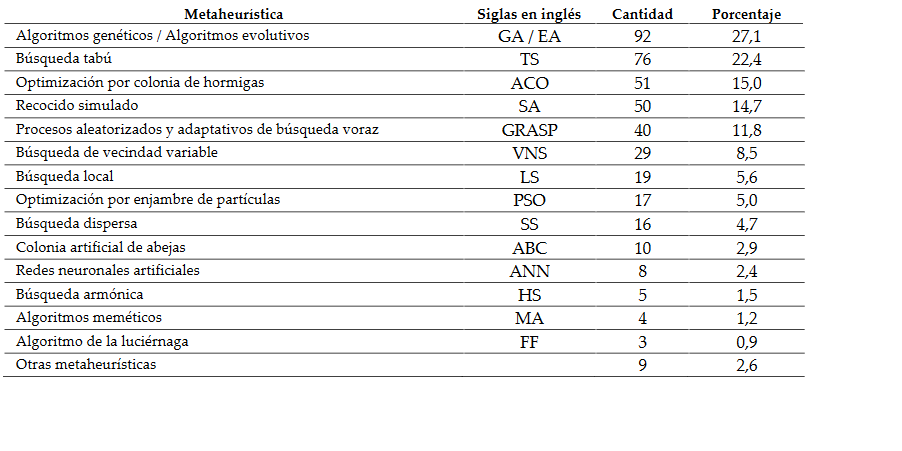
\includegraphics[scale=0.8]{./Graphics/EoAmetaheuristicas.png}
		\caption{Relación de artículos y tipos de metaheurística empleada} \cite{EOAgomez2014metaheuristicas}.
		\label{EoAmetaheuristicas}
	\end{figure}
	
	No obstante, mientras se siguen desarrollando las metaheurísticas en la resolución de problemas, ya sea en la  creación  de nuevos algoritmos o mediante el perfeccionamiento de los ya existentes, ha surgido un nuevo concepto, se trata de las denominadas hiperheurísticas. Las mismas son definidas como métodos que inteligentemente controlan la selección de la heurística subordinada que debiera ser aplicada en cada punto de decisión del problema, dependiendo de las características del mismo y de las asociadas al espacio de búsqueda de la solución, mediante un mecanismo de aprendizaje. De esta forma, las hiperheurísticas buscan  tener una mayor vinculación entre la calidad de la solución y la rapidez de la implementación y la ejecución. Algunas de las metaheurísticas utilizadas por las hiperheurísticas son  la búsqueda  tabú  incremental, algoritmos genéticos, colonia de hormigas, recocido simulado incremental, entre otras. \\
	
	Otras de las técnicas usadas en la resolución de problemas de optimización combinatoria, son los algoritmos aproximados \cite{vasiliev2018algoritmos}. Se dice que un algoritmo es $\alpha$-aproximado \cite{johnson1974approximation}, si para un problema de minimización, computa una solución factible de costo a lo sumo $\alpha$-veces el costo óptimo en tiempo polinomial. A diferencia de las heurísticas, que encuentran buenas soluciones en un tiempo razonable pero no siempre calculable, los algoritmos aproximados se basan en encontrar soluciones cuyo tiempo de ejecución está acotado por una cota conocida.
	
	Entre las técnicas más usadas se encuentran los algoritmos golosos, la técnica de Baker para grafos planares y \emph{fractional local ratio}.
	
	Los algoritmos golosos son aquellos donde en cada iteración buscan maximizar el beneficio \cite{jungnickel2005graphs}. Las demostraciones de los factores de aproximación se basan muchas veces en relacionar directamente una solución óptima con la computada \cite{vasiliev2018algoritmos}.
	
	La técnica de Baker para grafos planares permite obtener algoritmos con factor $(1+ \epsilon)^2$ para todo $\epsilon > 0$ fijo. La idea es descomponer el grafo en componentes y resolver el problema de manera óptima en cada una de las mismas \cite{vasiliev2018algoritmos}.
	
	\emph{Fractional local ratio} es una técnica que se basa en encontrar una solución factible y una descomposición de los costos de forma que se puedan acotar los errores incurridos por la solución computada respecto a cada componente \cite{vasiliev2018algoritmos}.
	
	\subsection{Evaluación de Código}
	
	La calidad de una herramienta digital se establece en base a la escritura del código fuente y la arquitectura diseñada. Que una aplicación esté libre de fallos y que además facilite la comprensión en la lectura y reusabilidad del código resulta de gran importancia para su aprobación.
	
	En la actualidad existen numerosas herramientas que de alguna manera permiten expresar una métrica en cuanto a evaluación de un código. En lo adelante se hará mención de algunas de las mismas.
	
	\begin{itemize}
		\item SonarQube es una plataforma desarrollada en Java que permite realizar análisis de la calidad de código de forma automatizada, para lo cual se usan diversas herramientas de análisis estático de código fuente como Checkstyle, PMD o FindBugs que permiten obtener métricas que ayudan a mejorar la calidad. Resulta una herramienta de utilidad durante el testing de código en una aplicación \cite{SonarQube}.
		
		\item HP Quality Center es una herramienta de gestión de pruebas que tiene como objetivo el control de la calidad del software. Esta incluye la gestión de requisitos, gestión de pruebas y los procesos de negocio \cite{HPQualityCenter}.
	\end{itemize}
	
	Existen algunas métricas presentes en el código que nos permiten evaluar la calidad del mismo. Estas son ajenas al lenguaje de programación que se use. Algunas de las principales categorías son las siguientes \cite{callejas2017modelos}.
	
	\begin{itemize}
		\item Reusabilidad. Se refiere a la utilización en varios lugares del programa de un mismo código, evitando así volverlo a escribir y posibles errores. Un ejemplo sencillo de esto es la separación del programa en proyectos y las funcionalidades en métodos.
		
		\item Extensibilidad. Es la facilidad con que cuenta un producto para corregir defectos, cumplir nuevos requisitos y facilitar el mantenimiento futuro.
		
		\item Eficiencia. Se refiere al buen manejo de los recursos físicos del programa (la memoria) y el tiempo de ejecución, lo cual permite un mejor rendimiento.
	\end{itemize}
	
	Una herramienta que posibilita la evaluación automática de código, son los jueces online \cite{hernandez2017feedback}. La idea inicial de estos sistemas, fue la de servir como repositorio de problemas de programación que habían formado parte de concursos en competencias internacionales. Con el paso del tiempo, se han ido popularizando y en la actualidad se utilizan como herramientas didácticas que resultan de gran utilidad, las cuales permiten practicar y aprender algoritmia y métodos de programación de forma amena, llegando incluso a utilizarse en las aulas. Así, una situación común es que el profesor explique un tema e indique a sus alumnos qué ejercicios del juez pueden usar para practicar lo que ha contado. Los estudiantes envían una solución al problema reciben un veredicto positivo (solución correcta) o negativo (solución incorrecta).
	
	Una vez enviada la solución y teniendo los casos de prueba, solo resta comprobar si el resultado coincide o no. En general, aunque estos veredictos puedan variar entre un juez u otro (depende del conjunto de casos de prueba en incluso del lenguaje usado), se pretende expresar las mismas ideas. Los veredictos más comunes son:
	
	\begin{itemize}
		\item Error de compilación.
		
		\item Error en tiempo de ejecución.
		
		\item Tiempo de ejecución agotado.
		
		\item Error en la salida (difiere de la esperada).
		
		\item Problema aceptado. No hay error en la salida y se ejecuta en el tiempo establecido.
	\end{itemize}

	El usuario conocerá el veredicto del juez y podrá volver a realizar un  nuevo  envío  en  caso  de  no  haber  conseguido  un  veredicto  favorable. Lo anterior varía en dependencia del juez y de la modalidad que se esté usando (concurso, competencias, libre, entre otros). Cada juez puede  definir  sus  propios  criterios  al  respecto como pueden ser el número de intentos o la disponibilidad de los problemas.
	
	En este escenario, no es necesario tener un porciento de acierto para ``aprobar", pues se define el resolver exitosamente un problema cuando se vencen la totalidad de los casos, no hay diferenciación entre lo que pudiera ser una nota de 2, 3 o 4 en los exámenes ordinarios de programación. Por lo cual, los estudiantes carecen de retroalimentación al enviar una respuesta y recibir como resultado un veredicto de incorrecto.  \\
	
	Entre los principales jueces online podemos encontrar: 
	\begin{itemize}
		
		\item Caribbean Online Judge (COJ). Es un juez en línea para entrenar la programación de algoritmos con diferentes lenguajes \cite{COJ}.
		
		\item CodeChef. Es un sitio web de programación competitiva destinado a proporcionar una plataforma para la práctica y el perfeccionamiento de las habilidades de programación a través de concursos en línea \cite{codechef}.
		
		\item HackerRank es una empresa de tecnología que se enfoca en desafíos de programación competitivos, donde los desarrolladores compiten tratando de programar de acuerdo con las especificaciones proporcionadas \cite{hackerRank}.
		
		\item CodeSignal es una plataforma de evaluación basada en habilidades, cuya misión es descubrir, desarrollar y promover el talento técnico. Ofrecen desafíos a todos los niveles de habilidad con fines educativos y de reclutamiento \cite{codeSignal}.
		
	\end{itemize}
		
	\section{Resultados esperados, importancia y herramientas a utilizar}
	
		El objetivo general de esta tesis es la selección o ponderación de los casos de prueba que permita utilizarlos como medida de calidad para la evaluación de algoritmos. El objeto de investigación es la optimización combinatoria \cite{baykasouglu2014testing} abordada por meta-heurísticas \cite{OptimizacionCombinatoria} para ser aplicado en la definición de los casos de pruebas de las evaluaciones de los estudiantes de Programación en la Facultad de Matemática y Computación.
		
		El algoritmo a implementar y el uso de metaheurísticas y la aplicación o no de un modelo de optimización serán aspectos abordados a lo largo de este documento.
		
		Esta solución sería extensible a cualquier algoritmo de programación. Existe abstracción sobre los algoritmos a evaluar, pero se diseñó particularmente para los tipos de exámenes que se aplican en primer año. Con solo tener en cuenta otros factores como el tiempo de ejecución y la memoria consumida, se podría ampliar el marco de algoritmos evaluables por esta propuesta.
		
		La generación de casos será parte de trabajos futuros, no se proponen procesos o metodologías genéricas de generación automática de casos debido a su complejidad. Para la selección de casos de prueba, la generación realizada fue con fines experimentales.
		
		Quedaría por designar las métricas a utilizar para dicho fin. Cómo evaluar la aplicación y en base a cuáles aspectos se mide la calidad de estos sistemas de cómputo serán interrogantes a responder.

\chapter{Optimización Combinatoria}
	Los problemas de optimización combinatoria que involucran una extensa, pero finita, lista de posibles soluciones son muy comunes en la vida diaria. Por mencionar algunos, entre los más destacados se encuentran el diseño de redes de comunicación y la planificación de rutas de vuelo. Debido a la gran envergadura de estos problemas en cuanto a la cantidad de datos, resulta imposible enumerar las posibles soluciones y quedarnos con la mejor, pues no es factible en tiempo tal enumeración; incluso con los poderes de cómputo actuales, pues dicha lista crece de manera exponencial respecto al tamaño del problema.
	
	En los últimos 50 años se han desarrollado varios métodos de búsqueda, los cuales arrojan una solución factible cercana al óptimo del problema sin necesidad de explorar cada alternativa. Esto es lo que se conoce como Optimización Combinatoria. Los resultados han sido notorios, avances significativos en problemas de importancia para la ciencia como lo son el viajante y el enrutamiento de vehículos ya son palpables.
	
	Sin embargo, una buena parte de los problemas encontrados son computacionalmente intratables por su naturaleza o porque son lo suficientemente grandes como para impedir el uso de algoritmos exactos. En tales casos, los métodos heurísticos generalmente se emplean para encontrar soluciones buenas, pero no necesariamente óptimas. La efectividad de estos métodos depende de su capacidad para adaptarse a un ambiente particular, evitar el estancamiento en los óptimos locales y explotar la estructura básica del problema.
	
	Sobre la base de estas nociones, se han desarrollado diversas técnicas de búsqueda basadas en heurísticas, las cuales han mejorado la capacidad de obtener buenas soluciones a diversos problemas de optimización combinatoria. Algunos de los principales métodos son: Recocido Simulado \cite{dowsland2003diseno}, Búsqueda Tabú \cite{cunquero2003algoritmos}, Algoritmos Genéticos \cite{jimenez2009busquedas} y GRASP (Procedimiento Codicioso de Búsqueda Adaptativa Aleatoria) \cite{resende2003grasp}.
	
	\section{Metaheurísticas}
	
	Una heurística \cite{gonzalez2001evaluacion} es una técnica o método inteligente para realizar una tarea que no es producto de un riguroso análisis formal, sino del conocimiento experto sobre un tema a solucionar, la cual aporta soluciones con cierto grado de confianza y calidad. Un método heurístico es la parte práctica del concepto de heurística. Es un enfoque para la resolución de problemas que emplea un método práctico no garantizado para ser óptimo o perfecto, pero suficiente para los objetivos inmediatos.
	
	Las metaheurísticas \cite{yagiura2001metaheuristic} son una clase de métodos aproximados que están diseñados para resolver problemas difíciles de optimización combinatoria, en los que los heurísticos clásicos no son efectivos. Proporcionan un marco general para crear nuevos algoritmos híbridos combinando diferentes conceptos derivados de la inteligencia artificial, la evolución biológica y los procedimientos estadísticos. Generalmente se aplican cuando se desconoce de un algoritmo que resuelva de manera satisfactoria dichos problemas. Muchas veces lo anterior se debe a que no es factible explorar en su totalidad el espacio de soluciones en busca de un óptimo global, por lo que se emplean heurísticas o métodos aproximados. En los problemas de optimización combinatoria \cite{gandomi2013metaheuristic} usualmente se aplican metaheurísticas. \\
	
	La optimización combinatoria se basa en encontrar una configuración de bits (selección), respecto a la entrada del problema, que maximice o minimice una función objetivo específica. A los pasos intermedios anteriores a la solución se les denomina estados, y al conjunto de todos los estados candidatos se le llama espacio de búsqueda. La función objetivo, los estados y el espacio de búsqueda son definidos en función del problema.
	
	Existen metaheurísticas que mantienen un único estado actual durante cada instante de ejecución, el cual es actualizado en cada iteración. Este paso se conoce como función de transición. Otras metaheurísticas más sofisticadas mantienen, en vez de un único estado actual, un conjunto de estados candidatos. Así, la función de transición añade o elimina estados de este conjunto. Otros procedimientos pueden guardar información del óptimo actual, escogiendo el estado óptimo entre todos los óptimos locales obtenidos en varias etapas del algoritmo. \\
	
	Como se mencionó anteriormente, el espacio de búsqueda puede resultar extremadamente extenso o incluso infinito, por lo cual es necesario definir algunos criterios de parada para la ejecución del algoritmo. Entre los más comunes podemos encontrar el efectuar un número de iteraciones especificadas por el usuario, el alcance de un determinado tiempo de ejecución o el cumplimiento de una condición específica del problema.
	
	Existen muchos métodos heurísticos con comportamientos y objetivos diferentes, por lo que resulta complicado clasificarlos. Esto se debe en parte a que muchos de  ellos  han  sido  diseñados para un problema específico sin posibilidad de generalización o aplicación a otros problemas similares. Sin embargo, algunas situaciones pueden resultar tener un parecido en cuanto al tipo de idea a seguir para su solución, de ahí surge una especie de clasificación entre estos algoritmos.
	
	\begin{itemize}
		\item Métodos de Descomposición: son aquellos aplicables a problemas que se descomponen en varios subproblemas más sencillos de resolver que el original.
		
		\item Métodos Inductivos: la idea es generalizar versiones pequeñas o más sencillas al caso completo. Propiedades o técnicas identificadas en estos casos más fáciles de analizar pueden ser aplicadas al problema completo.
		
		\item Métodos de Reducción: consiste en identificar propiedades que cumplen principalmente las buenas soluciones e introducirlas como restricciones del problema.  El objetivo es restringir el espacio de soluciones al simplificar el problema. Se corre el riesgo de dejar fuera soluciones óptimas del problema original.
		
		\item Métodos Constructivos: se caracterizan por construir en cada paso una solución del problema. Usualmente son  métodos deterministas y suelen estar basados en la mejor elección en cada iteración.
		
		\item Métodos de Búsqueda Local: los  procedimientos  de  búsqueda o mejora local comienzan con una solución del problema y la mejoran progresivamente.  El procedimiento realiza en cada paso un movimiento de una solución a otra con mejor valor. El método finaliza cuando, para una solución, no existe ninguna solución accesible que la mejore.
	\end{itemize}
	
		Los métodos constructivos y los de búsqueda local resaltan entre los procedimientos metaheurísticos más empleados y con mejores resultados en la práctica, por lo que para la confección de nuestra propuesta fueron seleccionados algunos de los que resultan aplicables a nuestro problema. 
	
		\subsection{Greedy Randomized Adaptive Search Procedures} \label{sub:GRASP}
		GRASP \cite{GRASP} es una técnica de muestreo aleatorio iterativo. Tiene la invariante de que en cada iteración proporciona una solución factible al problema en cuestión. Hay dos fases dentro de cada iteración del algoritmo: la primera construye inteligentemente una solución a través de una función golosa aleatoria; la segunda aplica un procedimiento de búsqueda local a la solución construida con la esperanza de encontrar una mejora. Esto se repite mientras no se alcance una condición de parada, que pudiera ser el cumplimiento de un número de iteraciones o el alcance de un valor en la función objetivo.
		
		En la Figura \ref{GRASPgeneral} se muestra el procedimiento general del GRASP
		
		\begin{figure}[h]
			\centering
			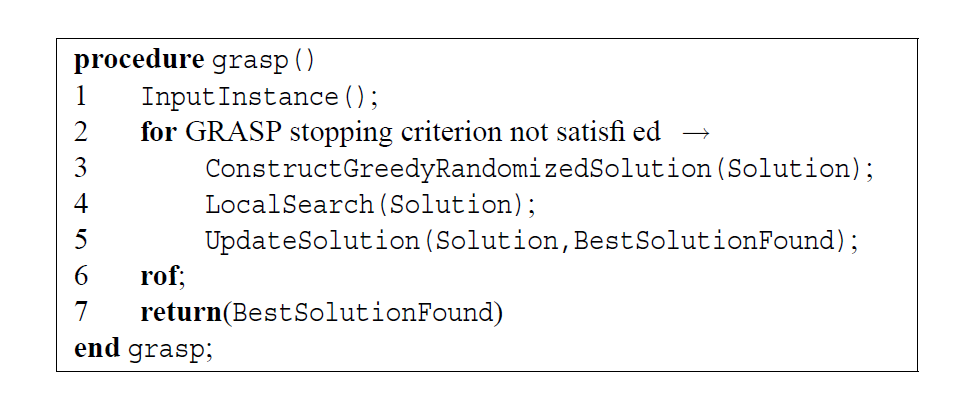
\includegraphics[width=10cm]{./Graphics/GRASPgeneral.png}
			\caption{Algoritmo GRASP \cite{binato2001greedy}}
			\label{GRASPgeneral}
		\end{figure}
		
		Ahora se construye iterativamente una solución factible. En cada iteración de construcción, la elección del siguiente elemento a agregar se determina respecto a una función golosa. Para reflejar los cambios provocados por la selección del elemento anterior, los beneficios asociados con cada elemento se actualizan en cada iteración. El componente probabilístico de un GRASP se caracteriza por elegir aleatoriamente uno de los candidatos de la lista, pero no necesariamente el mejor candidato. La lista de los candidatos se denomina lista de candidatos restringidos (RCL). Esta técnica de elección permite obtener diferentes soluciones en cada iteración GRASP.
		
		La Figura \ref{GRASPconstructionphase} muestra el pseudocódigo para la fase de construcción de GRASP.
	
		\begin{figure}[h]
			\centering
			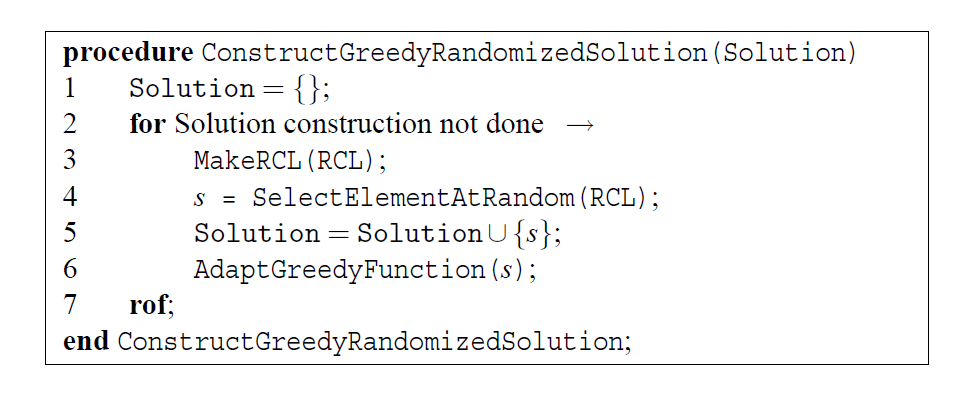
\includegraphics[width=10cm]{./Graphics/GRASPconstructionphase.png}
			\caption{Construcción de la solución GRASP \cite{binato2001greedy}}
			\label{GRASPconstructionphase}
		\end{figure}
	
		El algoritmo de búsqueda local es iterativo y reemplaza sucesivamente la solución actual por una mejor en la vecindad. Termina cuando no se encuentra una solución mejor en el vecindario. La clave del éxito para un algoritmo de búsqueda local consiste en la elección adecuada de una estructura de la vecindad, técnicas eficientes de búsqueda y la solución inicial.
		
		A continuación, la Figura \ref{GRASPlocal} muestra dicho procedimiento.
		
		\begin{figure}[h]
			\centering
			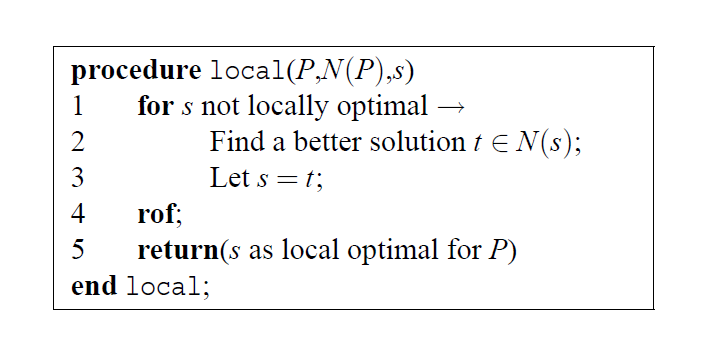
\includegraphics[width=10cm]{./Graphics/GRASPlocal.png}
			\caption{Búsqueda local GRASP \cite{binato2001greedy}}
			\label{GRASPlocal}
		\end{figure}
	
	\subsection{Recocido Simulado}
		Kirkpatrick, Gelatt y Vecchi (1983) e independientemente Cerny (1985) propusieron un nuevo enfoque para la solución aproximada de problemas de optimización combinatoria. Este enfoque, Recocido Simulado \cite{RecocidoSimulado} (Simulated Annealing) está motivado por una analogía con el comportamiento de los sistemas físicos en presencia de un baño de calor. El enfoque no físico puede verse como una versión mejorada de la técnica de optimización local o mejora iterativa, en la que una solución inicial se mejora repetidamente haciendo pequeñas alteraciones locales hasta que dicha alteración no produzca una mejor solución. El Recocido Simulado aleatoriza este procedimiento de una manera que permite movimientos ascendentes ocasionales (cambios que empeoran la solución), en un intento de reducir la probabilidad de quedar atrapado en una solución localmente óptima. El Recocido Simulado se puede adaptar fácilmente a nuevos problemas (incluso en ausencia de una comprensión profunda de los problemas mismos) y, debido a su aparente capacidad para evitar los óptimos locales deficientes, ofrece la esperanza de obtener resultados significativamente mejores.
		
		Para comprender el Recocido Simulado, primero se debe entender la optimización local. Se puede especificar un problema de optimización combinatoria identificando un conjunto de soluciones junto con una función de costo que asigna un valor numérico a cada solución. Una solución óptima es una solución con el mínimo costo posible (puede haber más de una solución de este tipo). Dada una solución arbitraria a tal problema, la optimización local intenta mejorar esa solución mediante una serie de cambios locales incrementales. Para definir un algoritmo de optimización local, primero se especifica un método para perturbar las soluciones para obtener otras. El conjunto de soluciones que se pueden obtener en uno de esos pasos a partir de una solución dada A se llama vecindad de A. El algoritmo luego realiza el ciclo simple que se muestra en la Figura \ref{OptLocalRS}, con los métodos específicos para elegir $S$ y $S'$ como detalles de implementación.
		
		\begin{figure}[h]
		\centering
		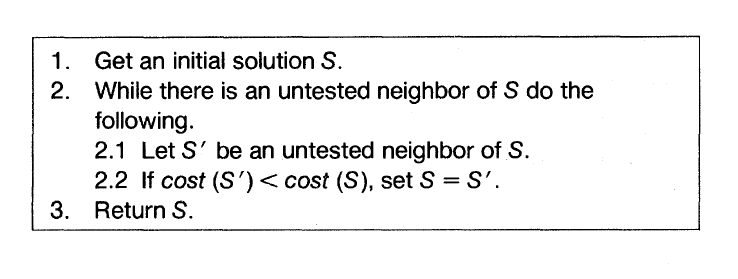
\includegraphics[width=10cm]{./Graphics/RecocidoSimuladoOptLocal.png}
		\caption{Optimización local \cite{RecocidoSimulado}}
		\label{OptLocalRS}
		\end{figure}
		
		Aunque S no necesita ser una solución óptima cuando finalmente se termina el ciclo, será localmente óptima ya que ninguno de sus vecinos tiene un costo menor. La esperanza es que localmente óptimo sea lo suficientemente bueno. \\
		
		La dificultad de la optimización local es que no tiene forma de retirarse de los óptimos locales poco atractivos. Nunca se pasa a una nueva solución a menos que la dirección sea cuesta abajo, es decir, a un mejor valor de la función de costo. El Recocido Simulado es un enfoque que intenta evitar dicho atrapamiento. Esto se realiza bajo la influencia de un generador de números aleatorios y un parámetro de control llamado temperatura. Como se implementa típicamente, el enfoque de Recocido Simulado involucra un par de ciclos anidados y dos parámetros adicionales, una relación de enfriamiento $r$, $0 < r <1$, y una longitud de temperatura entera $L$ (ver Figura \ref{RecocidoSimulado}). En el Paso 3 del algoritmo, el término congelado se refiere a un estado en el que no parece probable una mejora adicional en el costo ($S$).
		
		\begin{figure}[h]
		\centering
		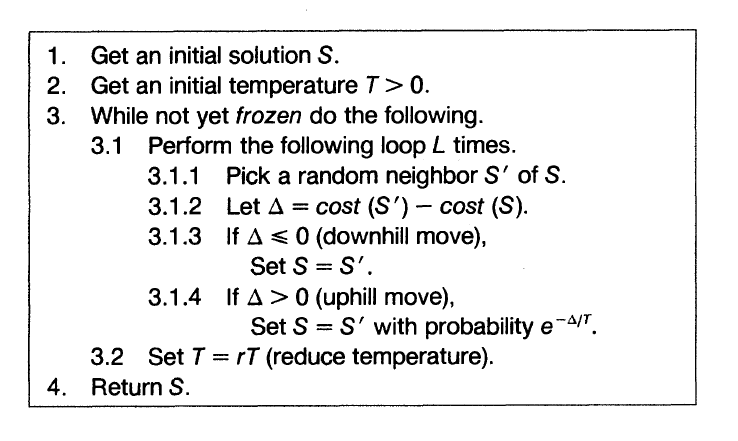
\includegraphics[width=10cm]{./Graphics/RecocidoSimulado.png} 
		\caption{RecocidoSimulado \cite{RecocidoSimulado}}
		\label{RecocidoSimulado}
		\end{figure}
		
		$e ^{-\Delta / T}$ será un número en el intervalo $(0, 1)$ donde $\Delta$ y $T$ son positivos. La probabilidad de que un movimiento cuesta arriba de tamaño $\Delta$ sea aceptado disminuye proporcionalmente a la temperatura y, para una temperatura fija $T$, los movimientos ascendentes pequeños tienen mayores probabilidades de aceptación que los grandes. Este método particular de operación está motivado por una analogía física.
		
	\subsection{Algoritmos Genéticos} \label{sub:Genetico}
		Un Algoritmo Genético \cite{AlgGen} consiste en un conjunto de soluciones codificadas, que hacen una analogía con los cromosomas.  Cada uno  de  estos tendrá asociado un ajuste o medida de aptitud, que expresa una métrica de su valor como solución al problema. En función de este valor se le darán más o menos oportunidades de ``reproducción". John Holland, investigador de la Universidad de Michigan, es uno de los principales precursores del desarrollo de los Algoritmos Genéticos. Sus trabajos a finales de la década de los 60 mostraron una técnica que imitaba en su funcionamiento a la selección natural \cite{melian2009algoritmos}.
		
		La reproducción en estos algoritmos puede darse de dos formas:
		
		\begin{itemize}
			\item Cruce: Se genera una descendencia a partir del mismo número de individuos (generalmente 2) de la generación anterior. 
			\item Copia: Un determinado número de individuos pasa sin sufrir ninguna variación directamente a la siguiente generación.
		\end{itemize}
	
		La Figura \ref{AlgoritmoeGenetico} muestra el funcionamiento de un algoritmo genético
	
		\begin{figure}[h]
			\centering
			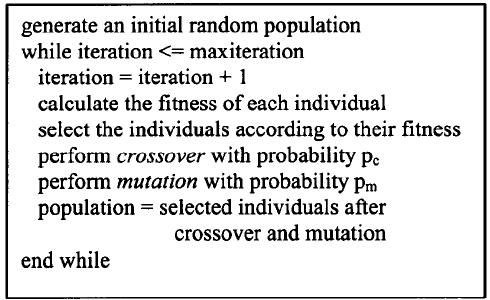
\includegraphics[width=9cm]{./Graphics/Genetic-Algorithm-pseudocode.png}
			\caption{Algoritmo Genético}
			\label{AlgoritmoeGenetico} \cite{ferentinos2002heuristic}
		\end{figure}
	
		Algunos de los criterios de parada pudieran ser:
		
		\begin{itemize}
			\item Se ha alcanzado una población con individuos lo suficientemente buenos para darle solución al problema.
			\item Ha convergido la población, lo cual quiere decir que la  media  de  bondad  de  la  misma  se aproxima a la bondad del mejor individuo.
			\item Se ha alcanzado el número de generaciones (iteraciones) especificado.
		\end{itemize}
	
		A este algoritmo se le han definido numerosas variantes. Una de las más extendidas es aplicar los operadores genéticos de cruce y copia directamente sobre la población genética \cite{AlgGen}. Pero en el caso de que se aplique cruce, no se puede insertar directamente la descendencia en la población, debido a que el número de individuos de la población se ha de mantener constante. Es decir, para permitir a los descendientes generados incorporarse a la población, se  han  de  eliminar  otros individuos. Trabajando con una sola población no se puede definir que la misma está llena, pues el número de sus miembros es constante. En este caso se pasará a la siguiente población cuando se hayan alcanzado un número determinado de cruzamientos especificados por el usuario, que deberán estar acordes al tamaño de la población.
		
\chapter{Diseño de la Propuesta}

	Para poder aplicar alguna metaheurística a la selección de casos de prueba, es necesario definir el espacio de búsqueda, así como las entradas, salidas y adaptaciones hechas a las implementaciones.
	
	Se provee al sistema de un conjunto inicial de casos de prueba brindados por el generador, los cuales inicialmente constituyen una solución, pues este problema de optimización no tiene restricciones, solo una función objetivo $f(x,y)$ a minimizar: \\
	
	$f(x,y) = |x - x_0| + |y - y_0|$ \label{fo}
	
	\begin{itemize}
		\item $x$: Porcentaje de acierto obtenido por la solución con nota 3.
		\item $x_0$: Porcentaje de acierto esperado de la solución con nota 3.
		\item $y$: Porcentaje de acierto obtenido por la solución con nota 4.
		\item $y_0$: Porcentaje de acierto esperado de la solución con nota 4.
	\end{itemize}

	La solución que brinde el algoritmo debe consistir en un subconjunto del conjunto inicial de casos de prueba, que debería tener una evaluación menor o igual que la inicial. Se ha de aclarar que la salida puede estar comprometida por el sesgo en los datos de entrada, es decir, que el conjunto que se reciba como entrada no sea una muestra representativa de la población de casos de prueba. \\
	
	Si se considera el problema de la multiplicación de polinomios, algunos aspectos a destacar serían los siguientes.
	\begin{itemize}
		\item La entrada al algoritmo serían 2 polinomios y su salida el resultado de su multiplicación.
		\item Se pasa como entrada a la propuesta un generador de polinomios y 3 respuestas al problema (implementaciones) asociadas a una nota (5, 4 o 3), además de los porcentajes de acierto esperados por cada solución. (5:100\%, 4:90\% y 3:75\% por ejemplo).
		\item La función objetivo será minimizar la sumatoria de los errores, donde error es el valor absoluto entre lo que se espera y lo obtenido en términos del porcentaje para cada nota.
	\end{itemize}

	La propuesta de solución deberá de los $n$ casos de prueba aleatorios proporcionados por el generador, reducirlos a un $k$ representativo que se ajuste a los porcentajes esperados por cada solución. Para ello se aplicarán algoritmos metaheurísticos descritos anteriormente. \\
	
	A continuación, se explican las adaptaciones hechas a los dos algoritmos implementados: GRASP y Genético, los cuales reciben la misma entrada y aplican un proceder diferente. La selección de estos dos se debe que, por un lado, el Algoritmo Genético tiene los mejores resultados en la práctica cuando se trabaja con problemas de optimización combinatoria, lo cual se evidencia en la Figura \ref{EoAmetaheuristicas} al ser el más utilizado. Por otro lado, GRASP, a pesar de figurar en la quinta posición, resulta intuitivo y fácil de implementar; además, puede servir de referencia para otras implementaciones, las cuales deberían obtener un mejor resultado.
	
	\section{Adaptación de GRASP}
		Como mencionábamos en el apartado \ref{sub:GRASP}, en cada iteración de GRASP Se hace una búsqueda local, la cual brinda otra solución factible al algoritmo. En este problema en particular, se tienen inicialmente los $n$ casos de prueba, de donde se selecciona un subconjunto que será la lista de candidatos de eliminar, los cuales representan una mejora (menor evaluación) de la función objetivo si no se les considerara en la solución final del problema. Esto se aprecia en la Figura \ref{GRASP. Candidatos}. Una vez conformada dicha selección se toma uno de la misma al azar y se retira, posteriormente se hace otra iteración del algoritmo pero ahora con un conjunto de tamaño $n-1$. La figura \ref{GRASP. General} muestra el funcionamiento general.
		
		\begin{figure}[!]
			\centering
			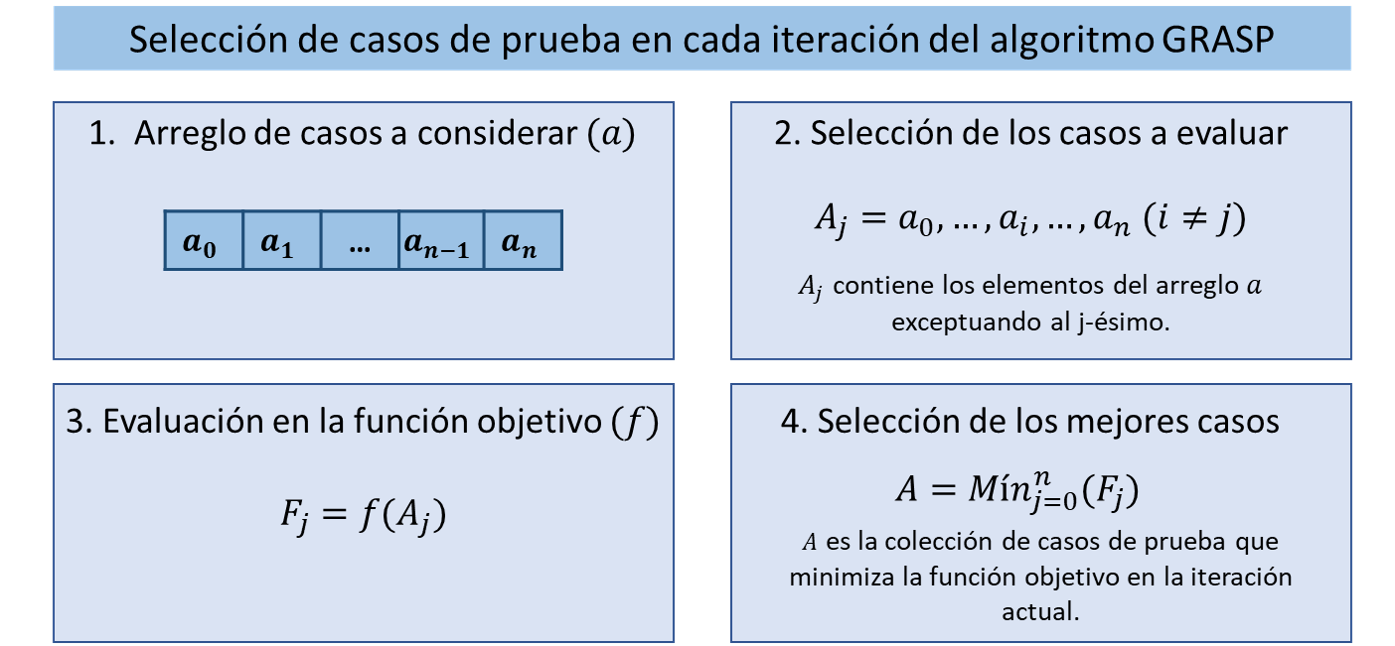
\includegraphics[width=12cm]{./Graphics/FiltrodeGRASP1.png}
			\caption{GRASP. Selección de Candidatos}
			\label{GRASP. Candidatos}
		\end{figure}
	
		\begin{figure}[!]
			\centering
			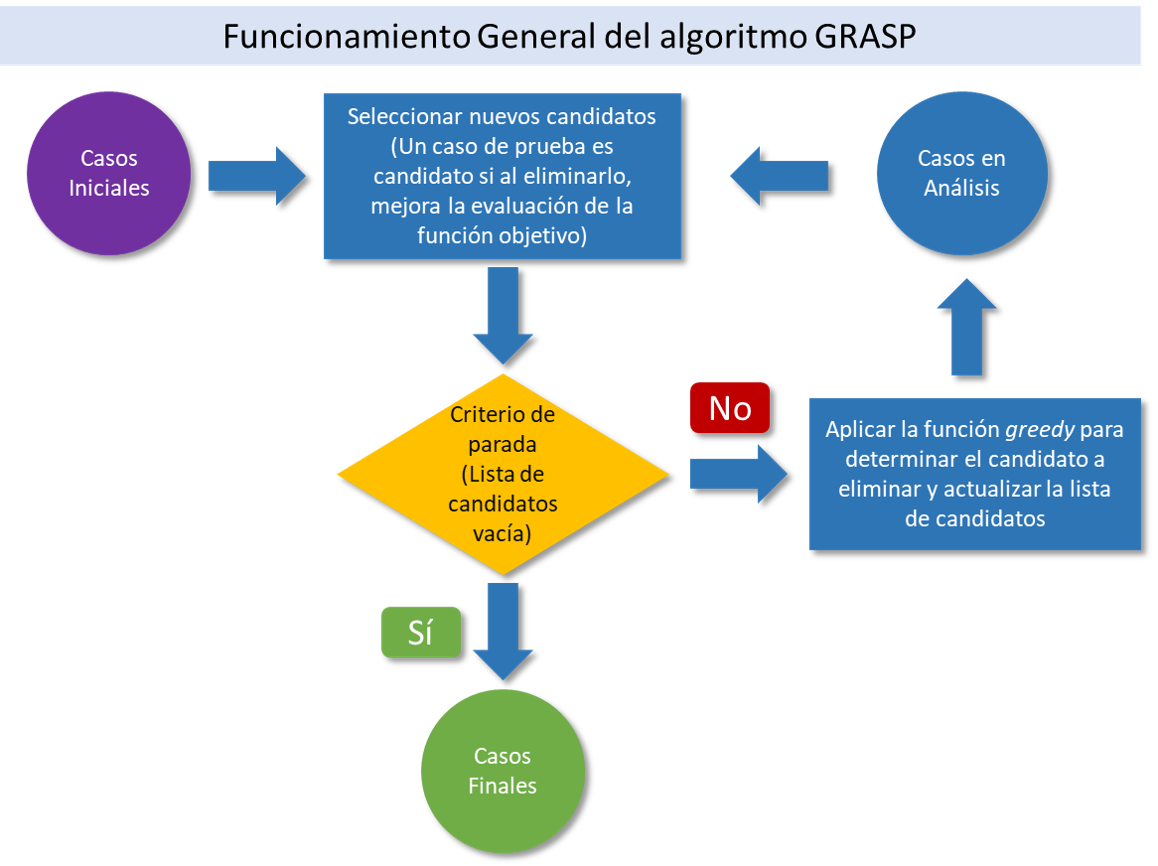
\includegraphics[width=10cm]{./Graphics/GraficoGRASP1.png}
			\caption{GRASP. Funcionamiento General}
			\label{GRASP. General}
		\end{figure}
		
		Como casos de parada se pueden encontrar los siguientes:
		
		\begin{itemize}
			\item Se ha alcanzado el valor esperado de la función objetivo.
			\item Se han cumplido un número de iteraciones especificadas.
			\item La lista de candidatos a extraer es vacía.
		\end{itemize}
	
		Para un mayor rendimiento de este algoritmo, se deben hacer varias pasadas con el conjunto inicial de los $n$ casos de prueba brindados por el generador, pues en la aleatoriedad de seleccionar el candidato a eliminar, puede que no siempre se esté caminando hacia el óptimo global. Por lo que varias corridas deberían lanzar un mejor rendimiento del algoritmo, el cual se quedará con la mejor de todas. La estimación del parámetro $k$ se hace de forma experimental y es posible que dos pasadas brinden la misma solución, pero esto último es muy poco probable.
		
	\section{Adaptación del Genético}
		En el Algoritmo Genético mencionado en el apartado \ref{sub:Genetico}, se definen varios operadores genéticos a efectuar sobre una población inicial de individuos, que serán métodos que reciben dos soluciones al problema. La entrada al procedimiento será el mismo subconjunto de tamaño $n$ que recibe GRASP. La diferencia está en que este último solo da pasos de tamaño $1$ en cada iteración, pues se visita una solución vecina que difiere en solo un caso ($1$ bit si se ven como máscaras booleanas sobre un conjunto). La Figura \ref{Genetico. General} muestra el funcionamiento general.
		
		\begin{figure}[h]
			\centering
			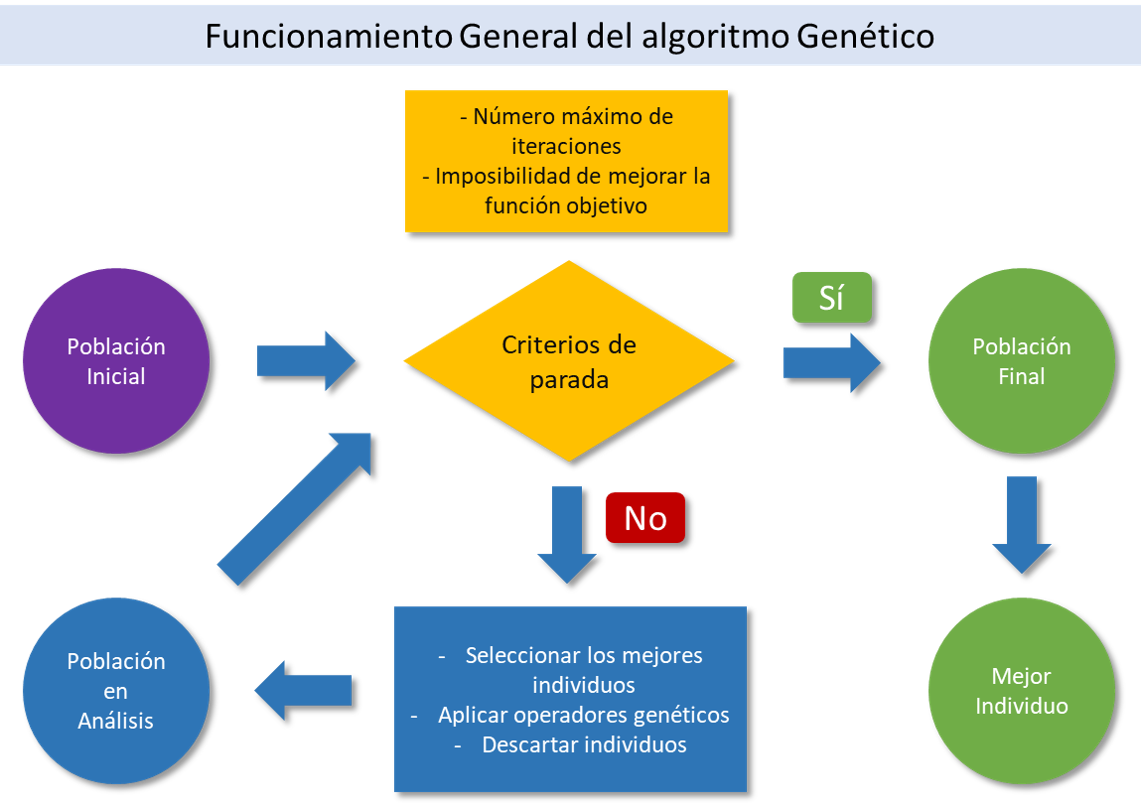
\includegraphics[width=10cm]{./Graphics/GraficoGenetico1.png}
			\caption{Algoritmo Genético. Funcionamiento general}
			\label{Genetico. General}
		\end{figure}
		
		La población inicial del algoritmo será de los $n$ casos iniciales, $k; k > 4$ configuraciones diferentes de bits sobre esos $n$. Una vez conformada, se procede a la selección de $4$ individuos que pudieran ser representativos.
		
		\begin{itemize}
			\item individuo $o_1$: el que mejor evalúa la función objetivo.
			\item individuo $o_2$: el segundo que mejor evalúa la función objetivo.
			\item individuos $r_1, r_2$: dos seleccionados de forma aleatoria.
		\end{itemize} 
	
		Operadores genéticos definidos donde $i1, i2$ son individuos de la población, o sea, soluciones al problema. La Figura \ref{OperadorGenetico} muestra un ejemplo de operador aplicado.
		
		\begin{figure}[h]
			\centering
			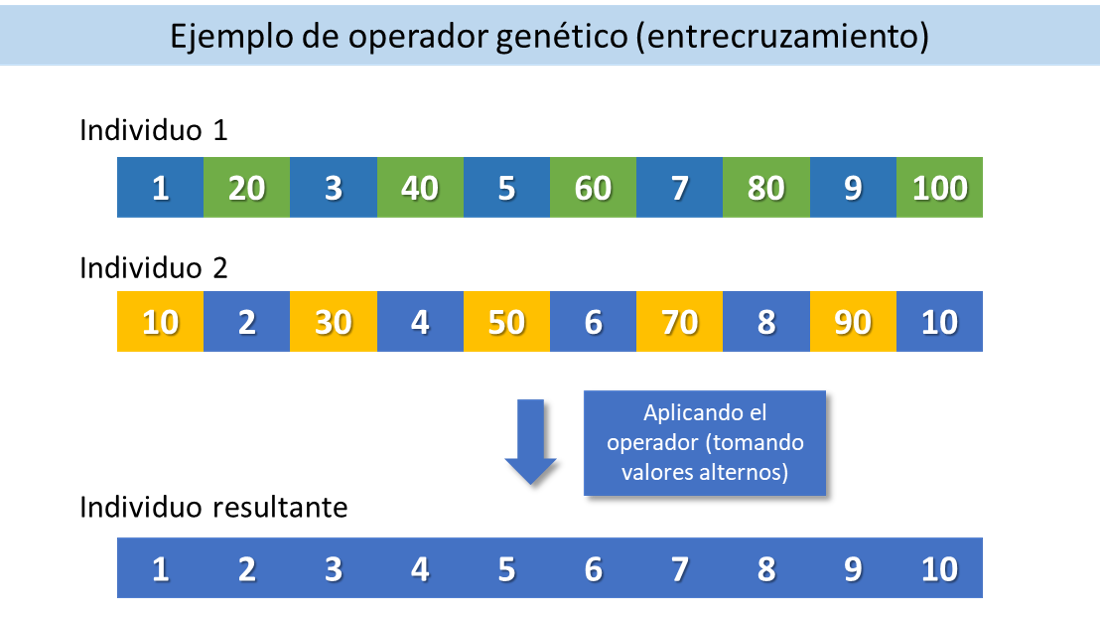
\includegraphics[width=10cm]{./Graphics/OperadordeGenetico.png}
			\caption{Operador Genético}
			\label{OperadorGenetico}
		\end{figure}
		
		\begin{itemize}
			\item operador $op_1(i_1, i_2)$: mezcla la primera mitad de $i_1$ con la segunda mitad de $i_2$.
			\item operador $op_2(i_1, i_2)$: mezcla de forma alternada $i_1$ e $i_2$.
			\item operador $op_3(i_1, i_2)$: unión de miembros aleatorios de $i_1$ e $i_2$.
			\item operador $op_4(i_1, i_2, p)$: mezcla el $p\%$ de $i_1$ con el $(1-p)\%$ de $i_2$.
		\end{itemize}
	
		Una vez definida la población inicial y los operadores genéticos, se procede a aplicar estos últimos sobre los $4$ individuos de la siguiente forma. Dados $o_1$ y $o_2$ se le pasan como parámetros cada operador genético, similar con $r_1$ y $r_2$. De esta forma se obtienen $8$ nuevos individuos, de los cuales se seleccionan los $4$ mejores y se añaden a la población. Esto se repite un número determinado de iteraciones y se devuelve el mejor individuo de la población, el cual minimiza la evaluación de la función objetivo.
		
		Note que en cada iteración del algoritmo, se aumenta en $4$ el número de soluciones, por lo que debe estar regulado el número de las mismas.
	
		De esta forma se intentan cubrir varios caminos que puedan llevar al óptimo y se dan pasos de más de tamaño $1$ (que difieran en más de un bit dos soluciones). Con un número de iteraciones lo suficientemente grande, este algoritmo debe acercarse a una buena solución del problema dado el balance entre exploración y explotación que posee.
		
		Aunque no se puede asegurar que los operadores genéticos definidos resuelvan el problema del estancamiento local, garantizan una aleatoriedad en la población que es necesaria para una buena exploración. Pudiera existir el mismo individuo repetido en la población, pero la variedad de operadores intenta cubrir la mayor cantidad de casos posibles.
	
\chapter{Resultados Obtenidos}

	Los resultados en cuanto a la eficacia de los algoritmos en reducir la evaluación de la función objetivo, fueron analizados en base a un mismo conjunto de casos de prueba en varias ejecuciones del algoritmo. Se utilizó la aplicación Visual Studio y el lenguaje de programación C\#. Esta elección se debe a las facilidades que ambos brindan para la confección de una solución a este problema. Pero pudiera haberse utilizado cualquier lenguaje de propósito general. 
	
	\section{Experimento 1}
	El problema analizado en particular fue el de multiplicación de polinomios: se reciben 2 arrays que representan coeficientes, según el índice que ocupan es el grado de la variable que acompañan. Se debe devolver un array resultante de la multiplicación de ambos. Dicho conjunto de pares de polinomios fue generado de manera aleatoria. \\
	
	En la tabla \ref{tab:IndicadoresGRASP123} se muestran algunos detalles de 3 ejecuciones distintas donde se aplica GRASP sobre el mismo conjunto, los casos están enumerados del $1$ al $n$. Dado el no determinismo inherente a la metaheurística empleada, los 3 subconjuntos obtenidos son distintos entre sí en cuanto a casos de prueba. Sin embargo cada ejecución tiene los mismos valores finales en los indicadores que se expresan en la tabla \ref{tab:IndicadoresGRASP123}.
	
	\begin{table}[h]
		\begin{center}
			\begin{tabular}{| l | c |} \hline
				Cantidad de casos iniciales & 250 \\
				Porcentaje inicial/esperado del 3 & 19.60/30 \\
				Porcentaje inicial/esperado del 4 & 95.20/90 \\
				Evaluación inicial de la f.o. & 15.60 \\ \hline
				Iteraciones del algoritmo & 87 \\ \hline
				Cantidad de casos finales & 163 \\
				Porcentaje final/esperado del 3 & 30.06/30 \\
				Porcentaje final/esperado del 4 & 92.63/90 \\
				Evaluación final de la f.o. & 2.699 \\ \hline
			\end{tabular}
			\caption{Indicadores iniciales y finales de las corridas 1, 2 y 3}
			\label{tab:IndicadoresGRASP123}
		\end{center}
	\end{table}

	Otros aspectos a destacar para comprender por qué sucede esto se muestran en la tabla \ref{tab:foGRASP123}, donde queda evidencia de la evaluación de la función objetivo a lo largo de las 3 corridas de GRASP sobre el conjunto de casos de prueba.
	
	\begin{table}[h]
		\begin{center}
			\begin{tabular}{| c | c |} \hline
				Iteración & f.o. \\ \hline
				0 & 15.600 \\
				1 & 15.502 \\
				2 & 15.403 \\
				... & ... \\
				43 & 10.53 \\
				44 & 10.39 \\
				45 & 10.24 \\
				... & ... \\
				85 & 3.030 \\
				86 & 2.800 \\
				87 & 2.699 \\ \hline
			\end{tabular}
			\caption{Valor de la función objetivo según las iteraciones}
			\label{tab:foGRASP123}
		\end{center}
	\end{table}
		
	En cada una de las 3 ejecuciones de GRASP se hicieron exactamente 87 iteraciones. Como resultado se eliminaron conjuntos de casos distintos, pero la evaluación de la función objetivo en cada paso se redujo de manera idéntica. \\
	
	Haciendo un análisis más profundo, dadas las peculiaridades del problema general a resolver, se pueden clasificar en 4 grupos los casos de prueba:
	
	\begin{itemize}
		\item tipo $uno$: son de la forma $(0, 0)$, donde ninguna implementación acierta el caso.
		\item tipo $dos$: son de la forma $(0, 1)$, donde solo acierta la implementación del 4.
		\item tipo $tres$: son de la forma $(1, 1)$, donde ambas implementaciones aciertan el caso.
		\item tipo $cuatro$: son de la forma $(1, 0)$, donde solo acierta la implementación del 3.
	\end{itemize}

	Debido a la información que se tiene ahora mismo sobre cada caso de prueba, el vector que se construye de estos es binario y de dimensión 2. Por tanto, el máximo número de tipos de casos posibles presentes en el problema general es 4.\\

	\textbf{Nota}: Por lo general, no existen los casos de la forma $(1, 0)$ donde acierte la implementación de 3 y la de 4 no. En la práctica puede que surjan de manera muy aislada. Se supone que una implementación de 4 debería acertar en los mismos casos que una de 3 y más, que no tenga un aspecto en el que quede por detrás de otra que obtenga una nota inferior. Sin embargo es posible que no se provea al sistema de una implementación de 4 puntos, por lo que los casos de la forma $(0, 0)$ y $(1, 0)$  serían los únicos presentes.\\
 
 	Una vez fijado el conjunto inicial de casos de prueba, ya la función objetivo toma un valor (ver definición de la misma en el Capítulo \ref{fo}). Si el porciento de acierto de la implementación de 3 fuese 75\% de un 80\% esperado y la de 4 fuese 90\% de un 95\% esperado. El algoritmo debe reducir en alguna medida los casos en que fallan ambas implementaciones, por lo cual la lista de candidatos a eliminar definida por GRASP en cada iteración serán solamente los casos de la forma $cero$. Por tanto de esa lista, que no va a variar en cuanto a grupos de casos, pues el tipo de un caso es invariable, se seleccionarán tantos casos a eliminar como la evaluación de la función objetivo lo permita (mientras mejore) y según la cantidad de casos del tipo objetivo presentes en el conjunto inicial.
 	
 	Por lo cual no importa cuál sea el conjunto inicial de casos de prueba, si se realizan varias ejecuciones de GRASP sobre el mismo, siempre se obtendrá un subconjunto final distinto en cuanto a casos de prueba pero con iguales evaluación de la función objetivo y cantidad de casos por tipo. En el cuadro \ref{tab:Tiposdecasos123} se aprecia lo anteriormente expuesto, solo se reducirá un tipo de caso particular en cada corrida. \\
 	
 	\begin{table}[h]
 		\begin{center}
 			\begin{tabular}{| c | c | c |} \hline
 				Tipo de caso & Cantidad Inicial & Cantidad Final \\ \hline
 				uno & 12 & 12 \\
 				dos & 189 & 102 \\
 				tres & 49 & 49 \\ \hline
 			\end{tabular}
 			\caption{Tipos de casos presentes en las corridas 1, 2 y 3}
 			\label{tab:Tiposdecasos123}
 		\end{center}
 	\end{table}
 
	Como se ha mencionado, los casos de prueba se generan de forma aleatoria, por lo que desde ese inicio se puede estar comprometiendo el buen funcionamiento del algoritmo. Recibir como entrada una muestra donde esté representado el universo de casos de prueba permite una mejor evaluación de la función objetivo, pues el algoritmo es capaz de desestimar aquellos casos que no son iguales desde el punto de vista físico pero sí a nivel de evaluación (combinación lineal uno de otro). Tener toda la gama de casos de prueba le brinda la posibilidad de hacer ajustes para poder minimizar la función objetivo de manera óptima. De lo contrario podría estar condenada (que no se minimice todo lo posible) desde el principio. Al no poder garantizar esto, es posible que el algoritmo no pueda encontrar la solución óptima al problema si no pertenece al subconjunto que se recibe como entrada. \\
	
	Sin embargo hay otros aspectos negativos inherentes al problema general que afectan el desempeño del algoritmo. Por ejemplo, la tipología de los casos de prueba. La información que se tiene es muy poca, solo se adquiere noción de en cuáles implementaciones acertó, no existe un criterio que permita comparar 2 casos de prueba en cuanto a ser significativo para una implementación u otra. En la práctica, existen casos de prueba que resultan muy triviales y deben ser resueltos fácilmente por todas las implementaciones de 3 puntos y otros que, aunque sencillos, no todos resuelven. Es decir, se pierde la relevancia entre los casos de prueba dentro de un mismo tipo. \\
	
	La idea de la evaluación de un caso de prueba basada en una implementación única es insuficiente e irreal. En un contexto ideal se tendría una cantidad de implementaciones efectivas por cada caso de prueba y un valor asociado a la bondad del caso. Eso hace que el vector pase de ser binario a continuo en el intervalo [0, 1] y entonces se podría diferenciar mejor los casos. Esta necesidad hace que surja del problema general, un nuevo problema que sería el enriquecer la manera de evaluar cada caso.
	
	Es necesario crear una especie de ``tribunal" donde hayan varios jueces (implementaciones) que juzguen qué tan significativo puede resultar un caso de prueba para ellos. Ante esta nueva inquietud surgen también 2 posibles soluciones a este nuevo problema: \\
	
 	Variante 1: Que el usuario proporcione varias implementaciones de cada nota. De esta forma ya estaría conformado el tribunal encargado desde el inicio. Sin embargo, resulta poco práctica. El objetivo de esta tesis es reducir a un conjunto representativo de casos de prueba dado un conjunto inicial e implementaciones de 3 y 4. Con ello se pondría fin al problema de generar estos casos a mano como se hace hasta ahora. Si esta variante se convierte en solución final, el usuario se vería sometido a un problema que resultaría igual, mayor o incluso imposible de resolver en algunas situaciones. Por lo que no es del todo factible. \\
	
	Variante 2: Añadir soluciones automáticamente según el grado de similitud con las soluciones ``canónicas" provistas por el profesor. Así se resuelve el problema de no tener que garantizar el jurado desde un inicio, pero por otro lado puede que este no se llegue a conformar nunca. Se necesita cierta variedad entre las soluciones, esto tal vez no sea posible encontrarlo debido a que entre las implementaciones candidatas, ninguna cumple los requisitos o por las características del problema particular que no lo permita. \\
	
	Vale destacar que la variante 2 también está condicionada por el espacio de búsqueda, muchas veces infinito. Por lo que resulta infactible su total exploración. Una vez más se insiste en la importancia de contar con una muestra representativa de la población en el conjunto inicial de casos de prueba, para un óptimo funcionamiento de las metaheurísticas empleadas y de las propuestas de solución a este nuevo problema generado. \\
	
	Hasta aquí se ha podido apreciar los resultados del algoritmo GRASP aplicado a un conjunto de casos de prueba, veamos a continuación sobre ese mismo conjunto, el comportamiento del algoritmo genético. La tabla \ref{tab:IndicadoresGen1} muestra algunos indicadores de una de las corridas.
	
	Se especificaron como criterios de parada el cumplir 200 iteraciones o el alcanzar una evaluación de la función objetivo menor a 1. La población inicial fueron 5 subconjuntos disjuntos de soluciones cuya unión genera los 250 casos iniciales, a los cuales se les aplicaron los operadores genéticos. Es importante que se le suministren los mismos casos al genético que a GRASP, para poder establecer una comparación en base a la misma entrada, pero por las especificaciones del algoritmo genético, se distribuyeron esos 250 casos en 5 grupos
	
	\begin{table}[h]
		\begin{center}
			\begin{tabular}{| l | c |} \hline
				Cantidad de casos iniciales & 250 \\
				Porcentaje inicial/esperado del 3 & 19.60/30 \\
				Porcentaje inicial/esperado del 4 & 95.20/90 \\
				Evaluación inicial de la f.o. & 15.60 \\ \hline
				Iteraciones del algoritmo & 60 \\ \hline
				Cantidad de casos finales & 41 \\
				Porcentaje final/esperado del 3 & 29.268/30 \\
				Porcentaje final/esperado del 4 & 90.24/90 \\
				Evaluación final de la f.o. & 0.9756 \\ \hline
			\end{tabular}
			\caption{Indicadores iniciales y finales}
			\label{tab:IndicadoresGen1}
		\end{center}
	\end{table}

	Entre las corridas que se hicieron, fue notorio el apreciar algunas que lograron reducir la evaluación de la función objetivo a 0. Esto podría inducir la conjetura de que sea posible llevarla a 0 si se alcanza un adecuado número de iteraciones y se elimina el criterio de parada de la evaluación de la función objetivo anteriormente expuesto. La tabla \ref{tab:foGen1} muestra la evaluación media y la menor de la función objetivo en algunas de las iteraciones entre los subconjuntos que conforman la población actual de soluciones. Se aprecia como dicho criterio de parada se cumplió e influyó en la obtención de un óptimo.


	\begin{table}[h]
		\begin{center}
			\begin{tabular}{| c | c | c |} \hline
				Iteración & Evaluación media & Menor evaluación. \\ \hline
				0 & 15.6 & 12 \\
				1 & 14 & 8 \\
				2 & 12.6 & 6 \\
				... & ... & ... \\
				30 & 10.32632 & 1.30435\\
				31 & 10.2714 & 1.30435\\
				32 & 10.23214 & 1.30435\\
				... & ... & ...\\
				58 & 9.47092 & 1.30435\\
				59 & 9.49476 & 1.30435\\
				60 & 9.425285 & 0.9756107 \\ \hline
			\end{tabular}
			\caption{Valor de la función objetivo según las iteraciones}
			\label{tab:foGen1}
		\end{center}
	\end{table}

	El conjunto resultante de casos fue de tamaño 41 en esta corrida. Los casos según la clasificación en tipos definida anteriormente se muestran en la tabla \ref{tab:IndicadoresGen1}. Esta vez no todas las corridas arrojaron igual cantidad de tipos de casos ni idéntica cardinalidad del conjunto final.

	\begin{table}[h]
		\begin{center}
			\begin{tabular}{| c | c | c |} \hline
				Tipo de caso & Cantidad Inicial & Cantidad Final \\ \hline
				uno & 12 & 4 \\
				dos & 189 & 25 \\
				tres & 49 & 12 \\ \hline
			\end{tabular}
			\caption{Tipos de casos presentes en el conjunto final}
			\label{tab:TiposdecasosGen1}
		\end{center}
	\end{table}

	El rendimiento de ambos algoritmos en el experimento 1 se muestra en la Figura \ref{CallsMP}
	
	\begin{figure}[h!]
		\centering
		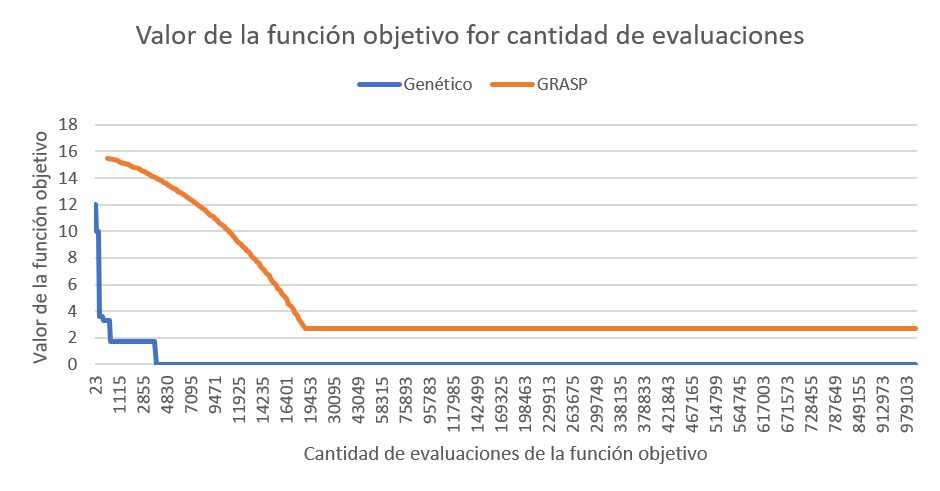
\includegraphics[width=10cm]{./Graphics/Calls-MP.png}
		\caption{Rendimiento Experimento 1}
		\label{CallsMP}
	\end{figure}

	\section{Experimento 2}
		Para probar estas metaheurísticas con casos reales se seleccionó el problema Anagramas, el cual fue aplicado en el curso 2018-2019 como primer examen de programación en la facultad de Matemática y Computación de la Universidad de La Habana. El mismo consiste en dado un $string$ $s$, obtener la cantidad de pares de $substrings$ de $s$ que son anagramas entre sí. Un anagrama es una palabra que resulta de la transposición de letras de otra palabra. Dicho de otra forma, una palabra es anagrama de otra si las dos tienen las mismas letras, con el mismo número de ocurrencias. Un $substring$ es una secuencia contigua de caracteres de al menos longitud uno.
		
		\begin{table}[h]
			\begin{center}
				\begin{tabular}{| l | c |} \hline
					Cantidad de casos iniciales & 3066 \\
					Porcentaje inicial/esperado del 3 & 82.84409/80 \\
					Porcentaje inicial/esperado del 4 & 98.63013/95 \\
					Evaluación inicial de la f.o. & 6.474228 \\ \hline
					Iteraciones del algoritmo & 436 \\ \hline
					Cantidad de casos finales & 2630 \\
					Porcentaje final/esperado del 3 & 80/80 \\
					Porcentaje final/esperado del 4 & 98.40304/95 \\
					Evaluación final de la f.o. & 3.403038 \\ \hline
				\end{tabular}
				\caption{Indicadores iniciales y finales. GRASP aplicado a Anagramas}
				\label{tab:IndicadoresAnaGRASP1}
			\end{center}
		\end{table}
	
	\begin{table}[h]
		\begin{center}
			\begin{tabular}{| l | c |} \hline
				Cantidad de casos iniciales & 3066 \\
				Porcentaje inicial/esperado del 3 & 82.84409/80 \\
				Porcentaje inicial/esperado del 4 & 98.63013/95 \\
				Evaluación inicial de la f.o. & 6.474228 \\ \hline
				Iteraciones del algoritmo & 10000 \\ \hline
				Cantidad de casos finales & 468 \\
				Porcentaje final/esperado del 3 & 79.91453/80 \\
				Porcentaje final/esperado del 4 & 96.5812/95 \\
				Evaluación final de la f.o. & 1.666672 \\ \hline
			\end{tabular}
			\caption{Indicadores iniciales y finales. Genético aplicado a Anagramas}
			\label{tab:IndicadoresAnaGen1}
		\end{center}
	\end{table}

	Entre las principales anotaciones sobre estas ejecuciones se destacan las siguientes:
	\begin{itemize}
		\item Alto número de casos finales resultantes de aplicar GRASP. Esto se debe a que en el algoritmo no existe el concepto de exploración de nuevos casos, el mismo solo recibe un conjunto y reduce según los tipos de casos existentes hasta que la próxima reducción no mejore la evaluación de la función objetivo. Por otro lado, la evaluación final de la función objetivo pudiera considerarse en el rango de aceptable siendo de 3.4.
		
		\item Alto número de iteraciones aplicadas en Genético. Aplicando la conjetura del caso de parada planteado anteriormente, se escogió de forma experimental un número de iteraciones que aporte un buen rendimiento del algoritmo.
		
		\item Buena reducción de la función objetivo resultante de ejecutar Genético. Este algoritmo sí maneja los conceptos de exploración y explotación al crear nuevos conjuntos de casos de prueba y conservar los conjuntos de mejor evaluación respectivamente. Por lo cual logra mejores resultados que GRASP.
	\end{itemize}
	
	Una vez obtenido el conjunto final de casos, utilizando el probador se le ejecutó cada caso a la solución de los estudiantes. Los resultados obtenidos por el algoritmo genético fueron invariantes al obtener igual cantidad de alumnos con notas de 2, 3, 4 y 5. La tabla \ref{tab:Notas} muestra la distribución de notas.
	
	Por lo general, en este tipo de exámenes de programación, resulta difícil ver una distribución homogénea de las notas, pues son problemas sencillos que tienen una solución clara. En algunos es posible determinar un tipo de caso de prueba muy específico que haga fallar las soluciones, entonces se ven más notas de 3 y 4.
	
	\begin{table}[h]
		\begin{center}
			\begin{tabular}{| c | c |} \hline
				Nota & Cantidad \\ \hline
				2 & 24\\ 
				3 & 0 \\
				4 & 1 \\
				5 & 25 \\ \hline
			\end{tabular}
			\caption{Distribución de las notas}
			\label{tab:Notas}
		\end{center}
	\end{table}

	Como observación, respecto a la cantidad de casos originales aplicados en el problema (70) y a la aplicada en esta experimentación (468), hubo un notado aumento en el porciento de acierto de los estudiantes. Esto se debe a que resuelven más casos satisfactoriamente pero que pueden resultar triviales o ser una combinación lineal entre sí, pero no la suficiente cantidad como para mejorar la nota. Por lo cual el tamaño del conjunto de casos finales, a pesar de lograr una buena evaluación de la función objetivo, debe tenerse en cuenta para futuras experimentaciones. \\
	
	El rendimiento de ambos algoritmos en el experimento 2 se muestra en la Figura \ref{CallsAna}
	
	\begin{figure}[h!]
		\centering
		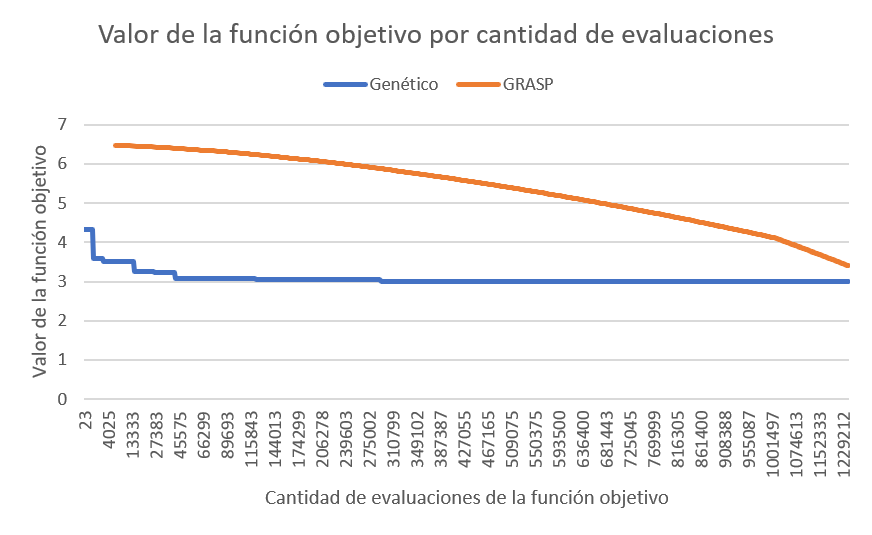
\includegraphics[width=10cm]{./Graphics/Calls-Anagramas.png}
		\caption{Rendimiento Experimento 2}
		\label{CallsAna}
	\end{figure}
	
	\section{Conclusiones}
	
	Tanto en la Figura \ref{CallsMP} como en la Figura \ref{CallsAna} se nota como GRASP se demora más en converger que Genético. Esto es resultado de la explotación presente que es lenta. Se realiza hacia vecinos de longitud 1 y los vectores son binarios y de tamaño 2, luego lo que hace es ajustar la cantidad de cada vector. Esto debe a las características del problema, en un ambiente estándar, lo que debiera pasar es que GRASP converja más rápido, mientras Genético se demore un poco más pero el óptimo encontrado por este último debería ser mejor.
	
	Quedó en evidencia mediante el experimento 1, que el algoritmo genético, al lograr una mejor reducción de la función objetivo, es más efectivo; al menos con las implementaciones actuales y en el espacio de búsqueda de los polinomios.
	
	Resulta poco sorprendente al anterior resultado, pues se hizo alusión que es la metaheurística más usada por los investigadores y en el diseño de la implementación, se plantearon operadores genéticos que garantizaron una aleatoriedad que permitió una adecuada exploración. Por lo tanto se visitaron muchas soluciones y se llegó a una que difiere poco del óptimo global y es aceptable como respuesta al problema.
	
	En el experimento 2 se reafirma que el algoritmo genético es muy útil, no presentó error (cambio de nota) respecto a las mediciones iniciales. Por lo cual, en estos tipos de problemas de optimización combinatoria a resolver con metaheurísticas, si lo que se desea es encontrar una solución tan cercana al óptimo como sea posible, entonces es recomendable aplicar el algoritmo genético. En caso de que se pueda contar con un margen de error, dada la simpleza en la implementación de GRASP, resulta muy factible de aplicar para la resolución de estos problemas.
	
	\section*{Recomendaciones y Trabajos Futuros}
	
	Como recomendaciones se tienen las siguientes:
	\begin{itemize}
		
		\item Hacer variaciones a los algoritmos implementados. Con esto se podrían lograr mejores resultados con un ajuste diferente en los parámetros o con otras implementaciones desde otro enfoque.
		
		\item Añadir nuevos algoritmos como Recocido Simulado o Búsqueda Tabú.
		
		\item Tener un conjunto de algoritmos y en dependencia del problema a resolver, escoger el que mejor se comporte en ese ámbito.
		
		\item Hacer un análisis más profundo de los operadores genéticos que pueda garantizar el no estancamiento local.
		
	\end{itemize}. 
	
	Como trabajo derivado de esta tesis se tiene:
	\begin{itemize}
		
		\item Hacer más extensible la calificación con notas.
		
		\item La generación automática de casos de prueba.
		
	\end{itemize}

	Este último elemento fue un tema que se tuvo en cuenta durante la experimentación. Como se ha hecho alusión anteriormente, una entrada representativa de casos de prueba, favorece el rendimiento de las metaheurísticas que se puedan aplicar. La generación hecha fue asistida, se trató de representar el universo de casos de prueba en dependencia del problema.
	

\bibliography{bibliography}
\bibliographystyle{ieeetr}

\end{document}